\documentclass{article}

\usepackage{lmodern}
\usepackage[english]{babel}

\usepackage{fontspec}
\defaultfontfeatures{Ligatures=TeX}

\usepackage{listings}
\usepackage{float}
\usepackage{hyperref}

\usepackage{graphicx}
\graphicspath{{assets/}}

\usepackage[
  style   = numeric,
  sorting = none,
]{biblatex}
\bibliography{paper}

\title{Analysing commit messages}

\begin{document}
  \maketitle

  \section{Introduction}
  \label{sec:introduction}

  With the rise of open source software, more and more big corporations
  incorporate free software in their stack. This also means that the amount of
  meaning-full software that is available online on platforms like GitHub
  \cite{github}, is ever increasing. GitHub, as the name already suggest,
  offers the ability to host Git repositories. Git is a distributed version
  control system \cite{git}. In this paper an effort has been made to analyse
  Git commits and gather information on their intended basic operation by
  looking at the message of the commit. To full-fill on the premise
  repositories of the top 10 most wanted programming language according to
  \cite{so-survey} have been investigated. To get a more accurate
  representation of each language, 100000 commits have been chosen. To enhance
  diversity, each repository is limited to 10000 commits. The analysis has been
  done in Python. Python is well suited for this project as it has rich support
  for natural language processing related tasks.

  \section{Methodology}
  As already alluded to in \autoref{sec:introduction} the goal of the project is to
  analyse commit messages. To achieve this repositories of the top 10 most
  wanted languages have been chosen, which are:


  \begin{figure}[H]
    \centering
    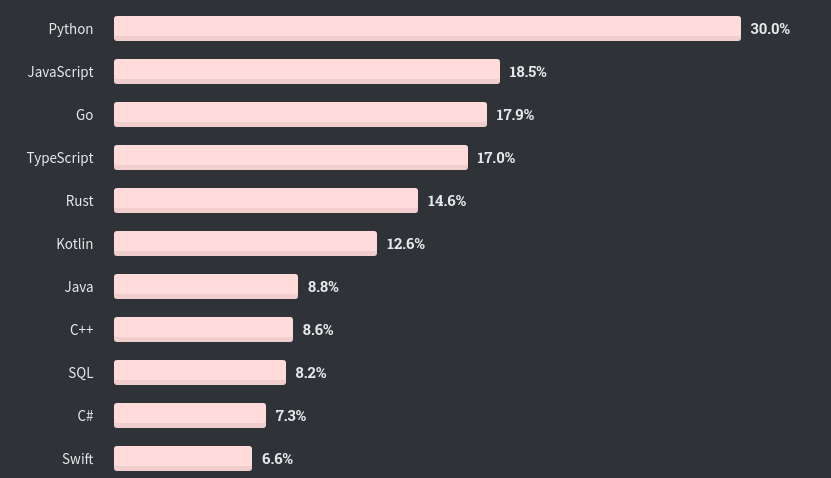
\includegraphics[width=\textwidth]{wanted_languages.png}
    \caption{top 10 most wanted languages}
    \label{fig:wanted_languages}
  \end{figure}
\end{document}
